%!TEX root = Thesis_main.tex

\chapter{Controller}
\label{chapter5}

\section{Introduction and Aim of the controller}

In this chapter the core of the developed controller will be presented. The goal of our research is to solve the mobile manipulation problem of trajectory tracking for handling and grasping tasks. The tasks we wish to perform are in general solved decoupling the controller in order to move the mobile robot in a defined position in order to have a fixed position of the base during grasping and to reduce uncertainties in end-effector position, and only then perform the grasping task with the manipulator. This approach is generally reliable since controlling independently the base of the robot and the arm with well-known techniques allows precision and robustness. Anyway, if we want to perform the tasks in a time-optimal way this approach is not suitable. The possibility to move within an environment during grasping operation to allow faster performance time is a goal desired not only in manipulation tasks but for many applications. Furthermore, the usage of a unique controller could allow exploiting the many degrees of redundancy to optimize other process variables such as manipulability or obstacle avoidance capability. What we have developed, is a unique controller able to deal with the whole mobile manipulator system. The controller we developed aims at solving some of the issues presented in Chapter \ref{chapter4} by means of a Nonlinear Model Predictive Control with a novel approach to solve the online optimization problem reducing the overall computational time. The choice of MPC controller has been made for many reasons: 

\begin{itemize}
\item by means of predicting the future states through the definition of a model it is possible to forecast the behaviour of the system. This approach becomes useful for obstacle avoidance and in manipulability maximization tasks;
\item it is an open framework that allows customized problems;
\item introducing constraints allows taking into account the feasibility set of the joint variable as well as control input limits;
\item being an Optimal controller allows the minimization of customized costs such as manipulability, control input effort etc...
\item it is generally used as a high-level controller, the low-level loops are in charge to track given high-level commands and deal with system dynamic;
\end{itemize}

In the next section the general NMPC structure for the mobile manipulation problem will be explained referring to a Nonholonomic vehicle and a 6 DOFs manipulator. Our novel approach to reduce computational time and the related stability proof will be discussed later on.

\section{Problem Definition}

In this section the variables of the system and the model used for the MPC problem will be defined. The choice of the kinematic model instead of the dynamic one has been made for different reasons:

\begin{itemize}
\item even if our approach allows to reduce computational time, the usage of the dynamic model introduces further complexity to forecast the future states, this slow down significantly the solving time;
\item because the control action of the kinematic model has been defined as velocities, it is easy to implement velocity constraints;
\item low-level motor controllers are usually in charge to track velocities with higher frequency loops, this hierarchical approach is widely diffuse in controlling complex robotic systems;
\item from a user point of view, kinematic variables allows a better understanding of what is happening on the real system;
\end{itemize}

\subsection{Model}

Consider the kinematic relation in \ref{dirkinMM} and the new state variables defined as:
\begin{equation} \label{state_control_def}
{x}(t) \in \mathbb{R}^n\ \  \textnormal{s.t.}\ \  {x}  = \left[ \begin{matrix} x_b \\ y_b \\ \theta_b \\ \Theta_1 \\ \Theta_2 \\ \Theta_3 \\ \Theta_4 \\ \Theta_5 \\ \Theta_6 \end{matrix} \right]\ \   \textnormal{and}\ \  {u}(t) \in \mathbb{R}^m\ \ \textnormal{s.t.}\ \ {u}=\left[ \begin{matrix} v \\ \omega \\ \dot{\Theta}_1 \\ \dot{\Theta}_2 \\ \dot{\Theta}_3 \\ \dot{\Theta}_4 \\ \dot{\Theta}_5 \\ \dot{\Theta}_6 \end{matrix} \right]
\end{equation}
where $x_b,\ y_b,\ \theta_b$ are the mobile base coordinates, $\Theta_1, \cdots ,\Theta_6$ are the joint values of the manipulator arm, $v, \ \omega$ are the base longitudinal and angular velocities, and $\dot{\Theta}_1, \cdots ,\dot{\Theta}_6$ are the manipulator joint velocities.
By means of these variables the nonlinear kinematic model of the Nonholonomic Mobile Manipulator can be defined as:
\begin{equation} \label{system_base}
	\dot{{x}}=f({x},{u})
\end{equation} 
where:
\begin{equation} \label{NLsystem}
	f({x},{u}) = \left[ \begin{matrix}
	G({x}) & 0 \\ 0 & I \end{matrix} \right]u
\end{equation}
and $G(x)$ is defined as in Equation \ref{Gmatrix_def}:
\begin{equation*}
G({x}) =  \left[
\begin{matrix}
\cos\theta_b & 0 \\
\sin\theta_b & 0 \\
0 & 1 
\end{matrix}
\right] 
\end{equation*}

The continuous time model in \ref{system_base} has been discretized by means of Runge Kutta 4 method, that results in:
\begin{equation} \label{system_base_d}
	{x}_{k+1}=f^+(x_k,u_k)
\end{equation}
Runge-Kutta method will be discussed more in details later on.

\subsubsection*{Notation:}
We will use the same notation as in Chapter \ref{chapter3}. Briefly recalling: ${x}_{k|i}$ is the state vector at time instant $i$ propagated starting from time instant $k$, and ${u}_{k|i}$ is defined in the same way. Moreover $f^+$ will define the discrete Runge-Kutta function approximating $f$.

\subsection{NLP definition}

As done in Chapter \ref{chapter3} we will set up a minimization problem considering a quadratic cost function in the form:
\begin{equation}\label{J_continua}
J({x}_{k|i},{u}_{k|i})=\sum_{i=1}^{N}l({x}_{k|i},{u}_{k|i})
\end{equation} 
where $l({x}_{k|i},{u}_{k|i})$ is a positive definite function dependent on the state and the control action. By including Equation \ref{system_base_d} and state and control feasibility boundaries the problem becomes: 
\begin{equation} \label{ourproblem_basic}
\begin{split}
		& min_{\textbf{u}_k}\ J({x}_{k|0},\textbf{u}_{k}) \\
		\textnormal{s.t.}\qquad
		&\ \ \ \ x_{k|i+1}=f^+(x_{k|i},u_{k|i}) \\
		&\ \ \ \ {x}_{k|i} \in \mathbb{X}\ \forall\ i=1,\dots,\ N  \\
		&\ \ \ \ {u}_{k|i} \in \mathbb{U}\ \forall\ i=0,\dots,\ N-1 \\
	\end{split}	
\end{equation}
where $\mathbb{X} = \lbrace {x_k}\in \mathbb{R}^n\ \textnormal{s.t.}\ {x}_{min}\leq x_k\leq x_{max} \rbrace$ is the feasible region of the state, $\mathbb{U} = \lbrace {u_k}\in \mathbb{R}^m\ \textnormal{s.t.}\ {u}_{min}\leq{u}\leq{u}_{max}, f^+(x_k,u_k) \in \mathbb{X} \rbrace $ and $\textbf{u}_k=[\ u_{k|0},\ u_{k|1},\ \dots,\ u_{k|N-1}\ ]$.
Note that the problem is discrete; we will refer at $T$ as the discretization time, so the time between $k$ and $k+1$ as well as the time between $i$ and $i+1$. \\
The problem defined in \ref{ourproblem_basic} is a standard NMPC problem that can be solved using well-known numerical optimization methods. The solution to the problem so defined will be $\textbf{u}^* \in \mathbb{R}^{m\times N}\ \textnormal{s.t.}\ \textbf{u}^* =[{u}^*_{k|0},\ {u}^*_{k|1},\ \dots,\ {u}^*_{k|N-1}]$. Even if, according to receiding horizon logic, only the first computed control action ${u}^*_{k|0}$ will be applied, the problem needs to be solved for all the prediction horizon. Because of that, the dimension of the problem is highly dependent on N. Considering our case, for example, we have $m=8$, so if we set $N=20$ the dimension of $\textbf{u}^*$ that has to be found is $8\times20=160$. The dependence of the problem dimension on the optimization horizon length generate restrictions on the choice of $N$. This is due to the increase in computational effort that may become too high to solve fast online applications like handling and grasping for mobile manipulators. A solution could be to bound the value of $N$ in order to keep the problem within a solvable dimension. However, the performance clearly increases as $N$ increases, allowing compliance with some constraints, like obstacle avoidance, over a longer period. For this reason, we introduced a parameterized control input approach to reduce the dependence of $N$ on the solving time, without losing the advantages of a longer prediction horizon.

\subsection{Parameterization}
The problem in \ref{ourproblem_basic} uses a control action defined as piece-wise constant that, as explained before, brings high computational cost dependence on $N$. To solve this issue we propose to express the control vector as a function of some parameters.
Let's consider a continuous time parametrization for the control input $u$ in \ref{state_control_def} defined as:
\begin{equation}
{u}(t)=F(t)p
\label{param_eq_cont}
\end{equation}
where $p \in \mathbb{R}^{N_p}$ s.t. $p=[\ p_1,\ p_2,\ \dots,\ p_{N_p}\ ]^T$. Considering this parameterization, the state equation of the system becomes:
\begin{equation}
	f(x,F(t)p)=\tilde{f}(x,p,t)
	\label{state_eq_par}
\end{equation}
Because the problem we aim to solve in \ref{ourproblem_basic} is defined as a discrete time problem, we will redefine Equation \ref{param_eq_cont} as discrete:
\begin{equation}\label{param_eq}
{u}_{k|i}=F(t_i)p_k
\end{equation}
where $t_i=(i-1)T\ \forall\ i=1,\ \dots,\  N$, and the matrix $F(t_i)$ is the base of the new space $\mathbb{R}^{N_p}$. The subscript $k$ for $p$ indicates the time instant the parameterization is referred to. \\
A good choice of the parameterization is made according to the physics of the variables to be parameterized. In \cite{kelly2013mobile} a parametric optimal approach is proposed, anyway, given that the variables to be controlled are longitudinal and angular velocities, a polynomial parameterization can fit the physical meaning requirement. The choice of the right parameterization to use will also be discussed in Section \ref{stabproof}. \\
\begin{figure}[h!]
	\centering
	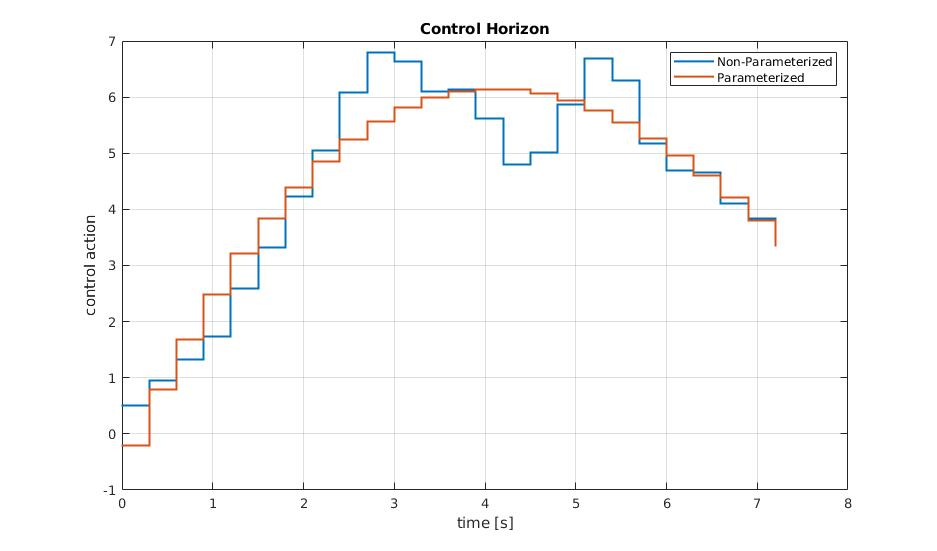
\includegraphics[scale=0.4]{param_horizon}
	\caption{Control input parameterization}
	\label{param_horizon}
\end{figure}
Considering a 3rd order Polynomial parameterization for the control inputs, as represented in Figure \ref{param_horizon}, each row of the ${u}$ vector can be expressed as a function of four parameters, for example $v=p_1t_i^3+p_2t_i^2+p_3t_i+p_4$. More in general ${u}_{k|i}$ is
\begin{equation}
{u}_{k|i}=\underbrace{\left[ \begin{matrix}
H_v(t_i)          & 0 & \dots      & 0  \\
0 &     H_\omega(t_i)      & \dots      & 0  \\
\vdots     & \vdots     & \ddots     & \vdots      \\
0 & \dots      & 0 &   H_{\Theta_6}(t_i)         \\
\end{matrix} \right]}_{F(t_i)} \left[ \begin{matrix} {p_v}_k \\ {p_{\omega}}_k \\ {p_{\Theta_1}}_k \\ {p_{\Theta_2}}_k \\ \vdots \\ {p_{\Theta_6}}_k \end{matrix} \right]
\end{equation}
where: 
\begin{equation}
\left[ \begin{matrix} {p_v}_k \\ {p_{\omega}}_k \\ {{p}_{\Theta_1}}_k \\ {{p}_{\Theta_2}}_k \\ \vdots \\ {{p}_{\Theta_6}}_k \end{matrix} \right] = \left[ \begin{matrix} {p_1}_k \\ {p_2}_k \\ {p_3}_k \\ \vdots \\ {p_{32}}_k \end{matrix} \right]\ \ \textnormal{and }\ \ H_*(t_i)=[\ t_i^3\ \ t_i^2\ \ t_i\ \ 1\ ]
\end{equation}
where $H_*(t_i)$ indicates each element on the diagonal of $F(t_i)$. Note that the value of $H_*(t_i)$ varies along the prediction horizon depending on the $i$th time instant. 

%%%%%%%%%%
Now, to discretize the continuous system in \ref{state_eq_par} we will use Runge-Kutta 4, so defining: 
\begin{equation*}
\begin{split}
    &k_1 = \tilde{f}(x_{k|i},p_k,t_i) \\
	&k_2 = \tilde{f}(x_{k|i}+k_1\frac{T}{2},p_k,t_i+\frac{T}{2}) \\
	&k_3 = \tilde{f}(x_{k|i}+k_2\frac{T}{2},p_k,t_i+\frac{T}{2})\\
	&k_4 = \tilde{f}(x_{k|i}+k_3T,p_k,t_i+\frac{T}{2})\\
\end{split}	
\end{equation*}
The new state equation becomes:  
\begin{equation}\label{state_eq_param}
\begin{split}
	x_{k|i+1}&=x_{k|i}+\frac{T}{6}(k_1+2k_2+2k_3+k4) \\
	&=\tilde{f}^+(x_{k|i},p_k,t_i)
\end{split}
\end{equation}
where $\tilde{f}^+$ denotes now the discretized parameterized state equation.
By applying the change of variables of Equation \ref{param_eq} into the problem formulation in \ref{ourproblem_basic} we obtain:
\begin{equation} \label{ourproblem_param}
\begin{split}
		& min_{p_k}\ J({x}_{k|0},p_k) = \sum_{i=1}^{N}\tilde{l}({x}_{k|i},p_k) \\
		\textnormal{s.t.}\qquad
		&\ \ \ \ x_{k|i+1}=\tilde{f}^+(x_{k|i},p_k,t_i) \\
		&\ \ \ \ {x}_{k|i} \in \mathbb{X}\quad \forall i=1,\dots, N  \\
		&\ \ \ \ p_k   \in \mathbb{P}\ \\
	\end{split}	
\end{equation}
where $\mathbb{P} = \lbrace p\in \mathbb{R}^{N_p}\ \textnormal{s.t.}\ F(t_i)p \in \mathbb{U}\quad \forall i = 1, \dots, N-1 \rbrace $ and $\tilde{l}$ is the stage cost $l$ as in Equation \ref{J_continua} being expressed as a function of $p_k$ instead of ${u}_{k|i}$. By means of this substitution the problem has to be minimized with respect to $N_p$ parameters, whose number do not depend on $N$. As a matter of fact, using 3rd order polynomials as in the previous example, we have to minimize $J$ with respect to $32$ parameters for any length of the prediction horizon. Implementing this approach results in a faster solution of the optimization problem, and the possibility to enlarge significantly the prediction horizon. Anyway $N$ has to be chosen properly: increasing too much the prediction horizon may result in bad performances due to overconstraining of the control action. This effect, as well as a performance comparison with respect to traditional MPC will be discussed later on.
\subsection{Increasing-Weight Cost Function definition}

Once the problem has been defined in its general form we have to properly choose the cost function. In particular, the stage cost $\tilde{l}$ has to be defined. A common choice is to use a quadratic stage cost in order to have a positive definite cost function. Even if it is important to have a quadratic cost function for the stability of the controller, it is still possible to find suboptimal solutions (i.e. local minima) because of the nonlinearities of the system. We will define the stage cost $\tilde{l}$ as a sum of different contributions using increasing weights into the optimization horizon, 
\begin{equation}\label{costfunctionh}
J({x}_{k|0},p_k)=\sum_{i=1}^{N}\left(\frac{i}{N}\right)^b \left[ \sum_{j=1}^{5} h_j({x}_{k|i},p_k) \right]=\sum_{i=1}^{N}\left(\frac{i}{N}\right)^b h({x}_{k|i},p_k)
\end{equation} 
where $b \in \mathbb{N}$ is the exponent of the weight term. This approach allows, by means of increasing weighted stage costs, to assess the stability of the NMPC without the imposition of terminal constraints, as shown in \cite{alamir2018stability}. This aspect will be reviewed in detail in the following section.
The definition of the functions $h_j$ defines what we want to minimize. Because the aim of the controller is to track the trajectory of the end-effector solving the mobile manipulation problem, the following stage costs are defined:
\begin{itemize}

\item first of all, $h_1$ is the cost related to the end effector pose error defined as: 
\begin{equation}
\begin{split}
h_1 = \left[\begin{matrix} \xi_{k|i}-\xi_{{d}_{k|i}} \\ [1\ 1]^T-\Phi_{k|i} \end{matrix}\right]^T W_1\left[\begin{matrix} \xi_{k|i}-\xi_{{d}_{k|i}} \\ [1\ 1]^T-\Phi_{k|i}\end{matrix}\right]\textbf{}
\end{split}
\end{equation}
Defining:
\begin{equation} 
\xi_{k|i} = \left[ \begin{matrix} x_{{ee}_{k|i}} \\ y_{{ee}_{k|i}} \\ z_{{ee}_{k|i}} 
\end{matrix} \right] = \left[ \begin{matrix}
1 & 0 & 0 & 0 \\ 0 & 1 & 0 & 0 \\ 0 & 0 & 1 & 0
\end{matrix} \right]A_{{ee}_{k|i}}\left[ \begin{matrix}
0 \\ 0 \\ 0 \\ 1
\end{matrix} \right]
\end{equation} 
and
\begin{equation}
\Phi_{k|i}=\left[\begin{matrix}\vec{\vartheta}_{k|i}\cdot\vec{\vartheta}_{d_{k|i}}\\ \vec{\psi}_{k|i}\cdot\vec{\psi}_{d_{k|i}}
\end{matrix}\right] 
\end{equation}

where $A_{{ee}_{k|i}}$ is the rototranslation matrix of the end effector with respect to the global reference frame, which is a function of the state $x$;  $\vec{\vartheta}_{k|i}$ and $\vec{\psi}_{k|i}$ are the orientation vectors of the end effector (i.e. the first and the third columns of $A_{{ee}_{k|i}}$) and $W_1$ is the diagonal weighting matrix for cost $h_1$.

\item In order to maximize the manipulability a cost related to the manipulability of the system is defined as:
\begin{equation}
h_2 = W_2 \left( \frac{1}{\det({\mathcal{J}_{ee}}_{k|i}^T{\mathcal{J}_{ee}}_{k|i})} \right)^2
\end{equation}

where ${\mathcal{J_ee}}_{k|i}=[\ {\mathcal{J}_b(x)}_{k|i}\ {\mathcal{J}_a(x)}_{k|i}\ ]$ are the Jacobians which relates the end effector pose to the joints of the base and of the arm, respectively. Like before $W_2$ is a weighting term. As briefly mentioned in Chapter \ref{chapter4}, there are many other ways to express an index for the manipulability of the system. For example, another way this index can be described is with the sine of the elbow joint angle of the manipulator, since the manipulability depends mostly on that angle.
    
\item $h_3$ is the cost related to the base control effort defined as: 
	\begin{equation}
	        h_3=\left[ \begin{matrix} v_{k|i-1} \\ \omega_{k|i-1} \end{matrix}\right]^T W_3 \left[ \begin{matrix} v_{k|i-1} \\ \omega_{k|i-1} \end{matrix}\right]
	 \end{equation}
This cost is particularly useful since the higher it is, the less the controller will choose to make adjustments on the end effector position through motions of the base, given that its positioning system is less reliable than the manipulator's one.
\end{itemize}
We will introduce now other two terms that will be used according to the application and in moving the system from and towards the grasping area. Decoupling the problem with two different cost functions allows having a faster controller during the motion of the system when it is required to have high speeds, and to increase the complexity of the problem only inside a grasping area, where the system moves slower, to perform grasping. The two additional terms are:
\begin{itemize}
    \item $h_4$ will be used to consider the base positioning error with respect to a given planned trajectory $x_{d_{base}}$ to reach the grasping area:
        \begin{equation}
            h_4=[x_{base}-x_{d_{base}}]^T W_4 [x_{base}-x_{d_{base}}]
        \end{equation}
     \item $h_5$ will be used to control the arm in joint space, so to track a desired joint position ${x_d}_{arm}$:
    \begin{equation}
       h_5=[x_{arm}-{x_d}_{arm}]^T W_5 [x_{arm}-{x_d}_{arm}]
    \end{equation}
\end{itemize}
where $x_{base}$ and $x_{arm}$ are defined as in \ref{dirkinMM}.
This terms, allowing to directly compute the error without passing through the forward kinematics, simplify a lot the problem during the motion of the base allowing a faster computation of the control action.\\We have shown only few terms, but others can also be added to make the controller more completely defined or to make it choose a solution for the kinematic redundancy problem in a different way. 

\section{Stability Proof}\label{stabproof}

Once the NMPC problem has been formulated and the feasibility of the problem has been investigated as in Equation \ref{feasibility} guaranteeing the fulfillment of hard  constraints, its stability has to be assessed. The proof is very similar to what done in \cite{alamir2018stability} with few modifications: extending it to a tracking problem, requiring an additional assumption regarding the parameterization and including the fulfillment of state and control constraints.
We will consider now, for the stability proof, the tracking problem as a zero-reference tracking problem. In order to do that we will consider:
\begin{equation}\label{change_var}
    e_k=x_k-{x_d}_k
\end{equation}
and so, substituting \ref{change_var} in the state equation \ref{state_eq_param}, we can define:
\begin{equation} \label{NLsystem}
	\hat{f}^+(e_{k|i},p_k,{{x_d}_{k|i}},{{x_d}_{k|i+1}},t_i) = \tilde{f}^+(e_{k|i}-{x_d}_k,p_k,t_i)
\end{equation}
then the discrete error state equation becomes:
\begin{equation}\label{sys_eq_con_e}
    e_{k|i+1}=\hat{f}^+(e_{k|i},p_k,{{x_d}_{k|i}},{{x_d}_{k|i+1}},t_i)=\hat{f}^+(e_{k|i},p_k,t_i)
\end{equation}
Note that, for simplicity of notation, the system equation in \ref{sys_eq_con_e} has been expressed as a function of the state error ${e_{k|i}}$ and the parameters $p_k$ only, given that the desired states are known.\\
In this way the problem is moved to track a zero error reference and becomes: 
\begin{equation} \label{ourproblem_stab}
\begin{split}
		& min_{{p}_k}\ J({e}_{k|0},{p}_k) =\sum_{i=1}^{N}\left(\frac{i}{N}\right)^b\hat{h}(e_{k|i},{p}_{k}) \\
		\textnormal{s.t.}\qquad
		&\ \ \ \ e_{k|i+1}=\hat{f}^+(e_{k|i},p_k,t_i) \\
		&\ \ \ \ e_{k|i} \in \mathbb{E}\ \forall\ i=1,\dots,\ N  \\
		&\ \ \ \ {p}_k\   \in \mathbb{P}\ \\
	\end{split}	
\end{equation}
where $\mathbb{E} = \lbrace {e}\in \mathbb{R}^n\ \textnormal{s.t.}\ {e}_{min}\leq e\leq e_{max} \rbrace$ is the feasible region of the state error and $\hat{h}$ is the stage cost function in \ref{costfunctionh} considering the change of variables in Equation \ref{change_var}. Now, following the demonstration in \cite{alamir2018stability} we need to introduce some assumptions in order to assess stability of the controller. The proof will consider some modification of what done in \cite{alamir2018stability} to consider the parametrization of the control input. 

\paragraph{Assumption 1} Equations $\hat{f}: \mathbb{R}^n\times\mathbb{R}^{N_p}\times\mathbb{R}\rightarrow\mathbb{R}^n$ and $\hat{h}: \mathbb{R}^n\times\mathbb{R}^{N_p}\rightarrow\mathbb{R}$ are continuous with respect to $e$, $p$ and $t$, and $\hat{h}$ is a positive definite function. That means a function $\hat{l}:\mathbb{R} \to \mathbb{C}$ such that, given any real numbers $x_1,\ \dots,\ x_n$, the matrix $A={(a_{i,j})}_{i,j=1}^{n_i}$ with $a_{i,j}=\hat{l}(x_i-x_j)$ is positive semi-definite, i.e. that $x^TAx \ge 0$. 

\paragraph{Assumption 2} We will require that a set $\mathbb{E}_N\subset\mathbb{E}$ exists so that $\forall e \in \mathbb{E}_N $ the set:
\begin{equation*}
	\mathbb{P}_{e \to 0}:=\lbrace \ p \in \mathbb{P}\ \text{s.t.}\ e_{N}(e,p)=0\ \rbrace
\end{equation*} exist and is not empty, considering $e_{N}(e,p)$ as the state error forecasted at time step $N$ calculated solving the problem in \ref{ourproblem_stab}, propagating the system from $e$ with the input commands parameterized with $p$. With this assumption we state that at least one vector $p$ for which $e_{N}(e,p)=0$ exists, and therefore a solution to the problem can be found.

\paragraph{Assumption 3} Local control invariance is assumed in the neighborhood of the origin, i.e. there exist a $\bar{\rho} > 0$ such that:
\begin{equation}
	\begin{split}
		\forall \rho &\leq \bar{\rho},\ \forall e \in B_{\hat{h}}(\rho),\ \exists\ \tilde{p}\ 	 \textnormal{s.t.} \\
		&\hat{h}\left(\hat{f}\left(e,\tilde{p},t\right),\tilde{p}\right)-\hat{h}\left(e,p\right) \leq -q(e,p) 
		\label{ass3}
	\end{split}
\end{equation}
for some positive definite function $q$ that satisfy:
\begin{equation}
	q(e,p) \ge \gamma \hat{h}(e,p)
	\label{ass3_1} 
\end{equation}
for some $\gamma \geq 0$ and $\forall e \in \mathbb{E}_N$,
where $B_{\hat{h}}(\rho) \subset \mathbb{R}^n$ is defined as $B_{\hat{h}}(\rho) := \lbrace\ e \in \mathbb{E}\ |\ h(e) \leq \rho \rbrace$. This is a rather standard assumption simply meaning that $\hat{h}$ is a local Lyapunov function with decrease rate described by $q$, i.e. there exist a value of the control action for which the variation of the cost function is bounded. In general, if $\hat{h}$ and $q$ are positive definite quadratic functions, inequality \ref{ass3_1} is valid.\\

{REMARK:  } Since the definition of $\mathbb{E}_N$ requires that $p \in \mathbb{P}$, i.e. that $p$ is a feasible control action, from its definition, and that $B_{\hat{h}}(\rho)$ is such that $e$ is within boundaries, Assumption 3 guarantees recursive feasibility as in \ref{def_rec_feas} because the \ref{ass3} states $\forall e\ \in B_{\hat{h}}(\rho)$ and $\forall e\ \in\ \mathbb{E}_N$

\paragraph{Assumption 4}
We will require an extended control input parameterization vector $p:=[p_1,\ p_2,\ \dots,\ p_{N_p},\ \kappa]$, with $\kappa\in\mathbb{N}$ such that: 
\begin{equation}
\begin{split}\label{new_parameterization}
    u_{k|i}(p_k)=
        \begin{cases}
            F(t_i){p_k}\ \ \ \ \   &\textnormal{if } i\le\kappa \\
            \bar{u}=\arg \min_u \hat{h}^u\left(f^+(x_{k-1|N},u,t_i),u\right)\ \ &\textnormal{if } i> \kappa
        \end{cases}
    \end{split}
\end{equation} 
where $f^+$ has been defined in \ref{system_base_d} and $\hat{h}^u\left(f^+(x_{k-1|N},u,t_i),u\right)$ is the stage cost expressed directly as a function of $u$ without passing through the parameterization. Note that the expression of $\bar{u}$ does not depend on the parameters vector $p$, since what we are interested in is a single evaluation of the input and not a parameterized function.\\
Moreover we will require that the parameterization function \ref{new_parameterization} has to be translatable: given the optimal solution at time instant $k$ defined as $p_k^*=\left[ p_{k_1}^*,\ p_{k_2}^*,  \dots,\ p_{k_{N_p}}^*,\ \kappa^* \right]^T$ that corresponds to $  \textbf{u}_k^*=[\ u_{k|0}^*,\ u_{k|1}^*,\  \dots,\  u_{k|{N-1}}^*\ ]$, it is possible to obtain the parameter $\tilde{p}_{k+1}$ such that the correspondent control input is $  \tilde{\textbf{u}}_{k+1}=[\ u_{k|1}^*,\ u_{k|2}^*,\  \dots,\  u_{k|{N-1}}^*,\ \bar{u} \ ]$. This is better understandable looking to Figure \ref{param_translatability}: if at time instant $k$ the computed optimal solution is represented by the blue line, the suboptimal solution $\tilde{p}_{k+1}$ for the optimization problem at time instant $k+1$ is the one described by the same blue line followed by the red one ($\bar{u}$).
\begin{figure}[h!]
	\centering
	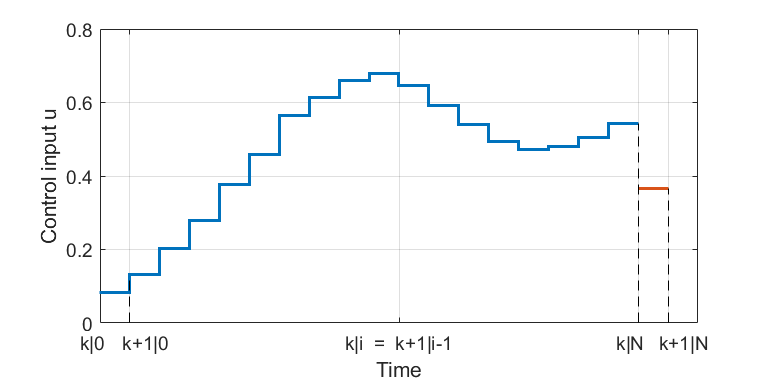
\includegraphics[scale=0.6]{IMMAGINI/trans_u.png}
	\caption{Translatability of the $F$ function}
	\label{param_translatability}
\end{figure}

\paragraph{Lemma 1} Under Assumption 1, $\forall e \in \mathbb{E}_N$, one has:
\begin{equation}
	\hat{h}(e_N(e,p^*)) \leq \eta\ c^b\ \ \  \textnormal{where    } c:=\frac{N-1}{N} < 1
 	\label{lemma1}
\end{equation}
for some $\eta > 0$ where $e_N(e,p^*)$ indicates the state at time instant N computed starting from time instant $e$ with the relative optimal solution $p^*$. \\

{PROOF:} The proof, as presented in \cite{alamir2018stability}, is done considering $p^0 \in \mathbb{P}_{e \to 0}$, which means to take a $p^0$ that allows reaching $e_N=0$ which is possible because of Assumption 1. By the definition of optimal solution we have: 
\begin{equation}
\begin{split}
	J(e,p^*)&\leq J(e,p^0) \\
	&\leq \sum_{i=1}^{N}\left(\frac{i}{N}\right)^b\hat{h}(e,p^0)
\end{split}
\end{equation}
and since by Assumption 1 we have $\hat{h}(e_N,p^0)=0$ we can remove the last term leading to:
\begin{equation}
	J(e,p^*)\leq \sum_{i=1}^{N-1}\left(\frac{i}{N}\right)^b\hat{h}(e,p^0)
\end{equation}
now, given that $\left(\frac{N-1}{N}\right)\sum_{i=1}^{N-1}\hat{h}(e,p^0) \geq \sum_{i=1}^{N-1}\left(\frac{i}{N}\right)^b\hat{h}(e,p^0)$:

\begin{equation}
	J(e,p^*)\leq \left(\frac{N-1}{N}\right)^b\sum_{i=1}^{N-1}\hat{h}(e,p^0)
\end{equation}
and considering:
\begin{equation}
 \eta \leq \textnormal{sup} \sum_{i=1}^{N-1}\hat{h}(e,p^0)
\end{equation}
leads to the proof of \ref{lemma1} because: 
\begin{equation}
h(e_N(e,p^*))\leq J(e,p^*) \leq \left(\frac{N-1}{N}\right)^b\eta = \eta c^b
\end{equation}

In order to assess stability it is required that the cost function $J({e}_{k|i},{p}_k)$ is proven to be a Lyapunov function as explained in Chapter \ref{chapter3}. 
We will consider now to have $p_k^*$ to which corresponds $\textbf{u}_k^*=[\ u_{k|0}^*,\ u_{k|1}^*,\  \dots,\  u_{k|{N-1}}^*\ ]$ as the optimal control parameterization at time instant $k$ and $\tilde{p}_{k+1}$ to which corresponds $\tilde{\textbf{u}}_{k+1}=[\ u_{k|1}^*,\ u_{k|2}^*,\  \dots,\  u_{k|{N-1}}^*,\ \bar{u} \ ]$ a suboptimal solution for time instant $k+1$.

So, considering the cost function related to $\tilde{p}_{k+1}$ as presented in \ref{ourproblem_stab} is it possible to state that:

\begin{equation*}
	\sum_{i=1}^{N}\left(\frac{i}{N}\right)^b \hat{h}({e}_{k+1|i},\tilde{p}_{k+1})=\sum_{i=1}^{N-1}\left(\frac{i}{N}\right)^b \hat{h}({e}_{k|i+1},p^*_{k})+\hat{h}^u\left(f^+(x_{k|N},\bar{u},t_i),\bar{u}\right)
\end{equation*}
and then:
\begin{equation*}
    J({e}_{k+1|0},\tilde{p}_{k+1})=\sum_{i=1}^{N-1}\left(\frac{i}{N}\right)^b \hat{h}({e}_{k|i+1},p^*_{k})+\hat{h}^u\left(f^+(x_{k|N},\bar{u},t_i),\bar{u}\right)
\end{equation*}
Now considering $j=i+1$ and a simplified notation $\hat{h}({e}_{k|i},p_{k}^*)=\hat{h}(e_{k|i})^*$, it follows: 
\begin{equation*}
    J({e}_{k+1|0},\tilde{p}_{k+1})=\sum_{j=2}^{N}\left(\frac{j-1}{N}\right)^b \hat{h}(e_{k|j})^*+\hat{h}^u\left(f^+(x_{k|N},\bar{u},t_i),\bar{u}\right)
\end{equation*}
Now rearranging the terms: 
\begin{equation*}
    \begin{split}
        J({e}_{k+1|0},\tilde{p}_{k+1})=&\sum_{j=2}^{N}\left[\left(\frac{j-1}{N}\right)^b-1\right]\left(\frac{j}{N}\right)^b \hat{h}(e_{k|j})^*+ \\
        &+\sum_{j=2}^{N}\left(\frac{j}{N}\right)^b \hat{h}(e_{k|j})^* + \hat{h}^u\left(f^+(x_{k|N},\bar{u},t_i),\bar{u}\right)
    \end{split}
\end{equation*}
Note that, subtracting the first stage cost at the optimal cost function at time instant $k$:   
\begin{equation*}
	\sum_{j=2}^{N}\left(\frac{j}{N}\right)^b \hat{h}(e_{k|j})^*=J({e}_{k|0},p_{k}^*)-\frac{1}{N^b}\hat{h}(e_{k|1})^*
\end{equation*}
So we get:
\begin{equation*}
    \begin{split}
        J({e}_{k+1|0},&\tilde{p}_{k+1})=J({e}_{k|0},p_{k}^*)-\frac{1}{N^b}\hat{h}(e_{k|1})^*+ \\ 
        &-\sum_{j=2}^{N}\left[1-\left(\frac{j-1}{N}\right)^b\right]\left(\frac{j}{N}\right)^b \hat{h}(e_{k|j})^*+ \hat{h}^u\left(f^+(x_{k|N},\bar{u},t_i),\bar{u}\right)
    \end{split}
\end{equation*}
And because $\forall j \in \lbrace2,\ \dots,\ N\rbrace$ holds that: 
$\left[ 1-\left(\frac{j-1}{N}\right)^b \right]\ge\left[ 1-\left(\frac{N-1}{N}\right)^b \right]= \phi(b)$. We can then say that: 
\begin{equation}\label{dim1}
    \begin{split}
        J({e}_{k+1|0},\tilde{p}_{k+1})\le &J({e}_{k|0},p_{k}^*) - \frac{1}{N^b}\hat{h}(e_{k|1})^*+ \\ 
        &-\phi(b)\sum_{j=2}^{N}\left(\frac{j}{N}\right)^b h(e_{k|j})^*+ \hat{h}^u\left(f^+(x_{k|N},\bar{u},t_i),\bar{u}\right)
    \end{split}
\end{equation}

Now according to Lemma 1, $e_{k|N}(p_k^*) \in B_{\hat{h}}(\eta c^b)$ and together with Assumption 3 implies that exist a value of $b$ for which it is possible to say:
\begin{equation}
\eta c^b \leq \bar{\rho}
\end{equation}
where $\bar{\rho}$ is the positive real called in Assumption 3. This is possible because, from the definition of $\rho$ in Assumption 3, we have that $\rho > 0$ and that $c>0$ for definition.
This means that \ref{ass3} holds for $e_{k|N}(p_k^*)$ and we can say that:
\begin{equation}\label{dim2}
    \hat{h}^u\left(f^+(x_{k|N},\bar{u},t_i),\bar{u}\right) \le \hat{h}(e_{k|N})^*-q(e_{k|N},p_k^*)
\end{equation}
because of the definition of $\bar{u}$ in Assumption 4. So, by applying this relation and Equation \ref{dim2} in Equation \ref{dim1} we obtain: 
\begin{equation*}
    \begin{split}
        J({e}_{k+1|0},\tilde{p}_{k+1})\le &J({e}_{k|0},p_{k}^*) - \frac{1}{N^m}h(e_{k|1})^*+ \\ 
        &-\phi(m)\sum_{j=2}^{N}\left(\frac{j}{N}\right)^b h(e_{k|j})^*+ h(e_{k|N})^*-q(e_{k|N},p_k^*)
    \end{split}
\end{equation*}
It is possible to note that: 
\begin{equation}
\phi(b)\sum_{j=2}^{N}\left(\frac{j}{N}\right)^b h(e_{k|j})^* \ge \phi(b)\hat{h}(e_{k|N})^*
\end{equation}
Then, using this and Equation \ref{ass3_1}:
\begin{equation*}
    \begin{split}
        J({e}_{k+1|0},\tilde{p}_{k+1})&\le J({e}_{k|0},p_{k}^*) - \frac{1}{N^b}\hat{h}(e_{k|1})^*+ \\ 
            &-(\phi(b)-1+\gamma)\ \hat{h}(e_{k|N})^*
    \end{split}
\end{equation*}

Noting that the stage cost is positive definite and that $\phi(b) \rightarrow 1$ for $b \rightarrow \infty$, for sufficiently high values of $b$ as can be seen in Figure \ref{phito1}, $J$ is a Lyapunov function as in \ref{Lyap_func}. In other words means that for sufficiently high values of $b$, $J({e}_{k|i},\tilde{p}_{k+1})\le J({e}_{k|i},p_{k}^*)$, and from what explained \ref{chapter3}, it follows that the closed loop system is asymptotically stable in $e=0$.
\begin{figure}[h!]
\centering
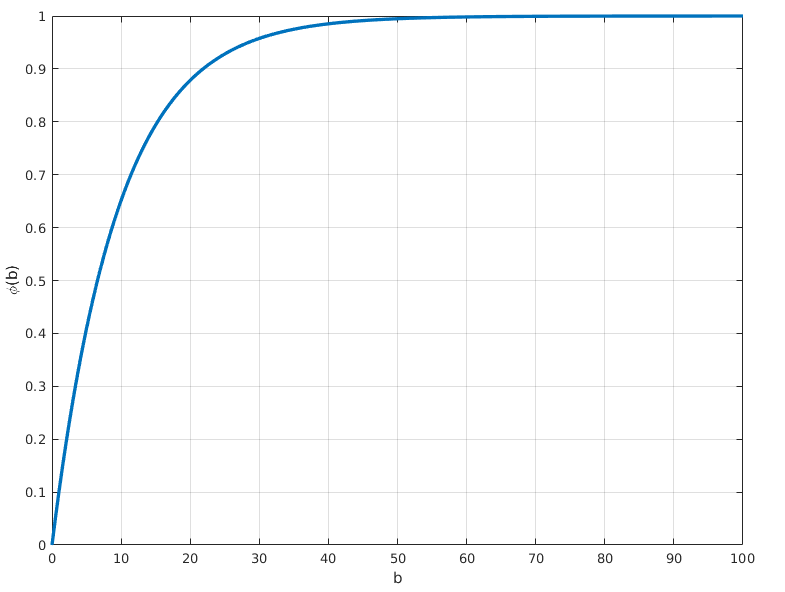
\includegraphics[scale=0.25]{IMMAGINI/phito1.png}
\label{phito1}
\caption{$\phi(b)$ value}
\end{figure}


\section{Constraints}
\fix{questa introduzione dei vincoli va rivista alla luce di come decidiamo la sezione prima}
Constraints will be introduced in order to properly define the problem taking into account feasibility configurations, maximum velocities and accelerations as well as to avoid self-collision of the system. Introducing constraints in the problem \ref{ourproblem_param} does not affect the stability proof since limiting state and control is equal to redefine accordingly sets $\mathbb{P}$ and $\mathbb{E}$ in Assumption 2 presented above. For example limiting joint speed for the arm is traduced in redefining the set $\mathbb{U}$, from which the set $\mathbb{P}$ is dependent and the proof in the previous section holds.

In particular, the constraint definition has been divided into: 

\subsubsection*{Joint position constraints}
	To limit the configurations of the robot into feasible sets and to avoid the arm to self collide there are different approaches. We decided to limit the possible positions of the joints of the arm into feasible ranges. This means to generate a set:
	\begin{equation}
		\mathbb{X}_{arm}:=x_{arm} \in \mathbb{R}^{6}\ \ \text{s.t.}\ \  {x_{arm}}_{min}\ \leq\ x_{arm}\ \leq\ {x_{arm}}_{max} 
	\end{equation}
	Applying this constraint into the MPC problem defined in Equation \ref{ourproblem_param} is straigthforward given that $\mathbb{X}_{arm}$ is a subset of $\mathbb{X}$.
\subsubsection*{Base position constraints}
	Contrary to the manipulator, self-collision of the base of the system is not possible and the joint $q_b$ could remain unconstrained. Anyway, the $x$ and $y$ coordinates of the base have been limited to define a region of operation for the Mobile Manipulator, see an example in figure \ref{xy_limits}. This constraint is particularly useful performing experiments defining a map of the surrounding environment. As before: 
	\begin{equation}
		\mathbb{X}^{x_{base}}:=x_{base} \in \mathbb{R}^3\ \ s.t.\ \  {x_{base}}_{min}\ \leq\ x_{base}\ \leq\ {x_{base}}_{max} 
	\end{equation}

	\begin{figure}[h!]
	\centering
	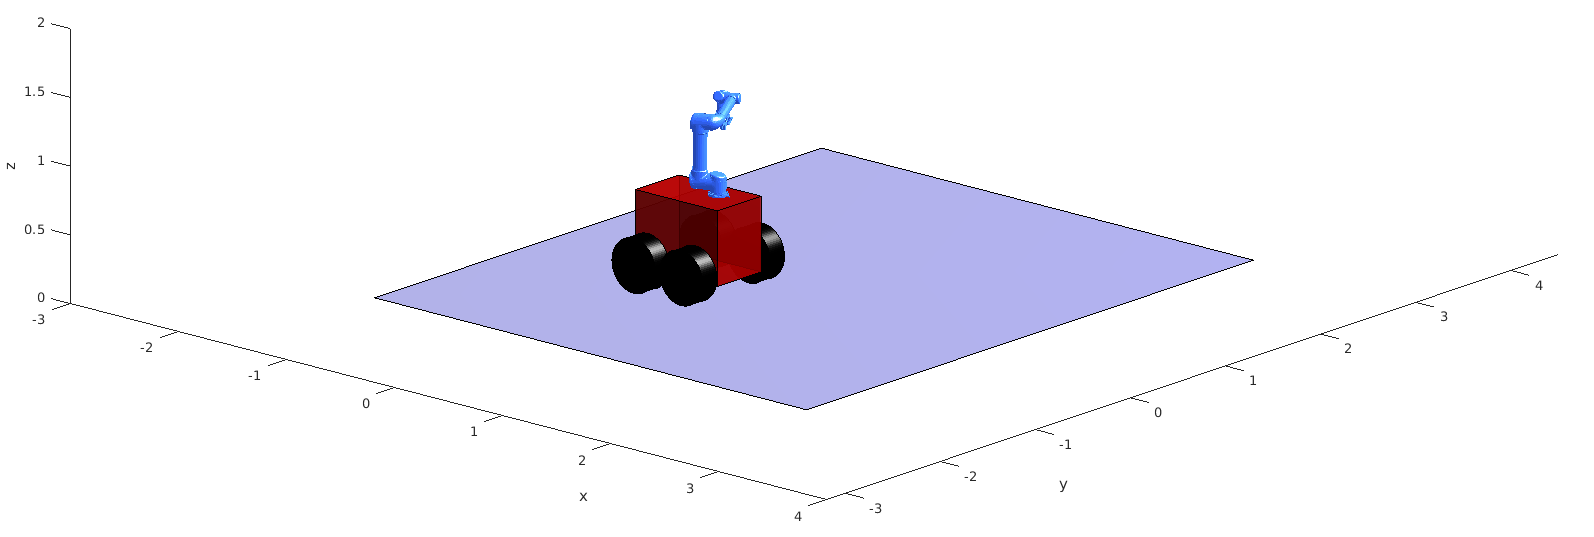
\includegraphics[scale=0.25]{IMMAGINI/xy_limits.png}
	\caption{Base $x-y$ limits}
	\label{xy_limits}
	\end{figure}

	Base and joint position constraints can be written in a compact form and for the entire prediction horizon redefining: 
	\begin{equation}
	\mathbb{X}:= x \in \mathbb{R}^{n}\ \ \text{s.t.}\ \  {x}_{min}\ \leq\ x\ \leq\ {x}_{max}
	\end{equation}

\subsubsection*{Velocity constraints}
	To take into account the maximum velcities allowed by the system, the control actions have been limited into minimum and maximum velocities according to manufacturer data in particular $\mathbb{R}^m$ have been redefined as:
	\begin{equation}
	\mathbb{U}:=\ {u}_{k|i} \in \mathbb{R}^m\ \ \textnormal{s.t.}\ \ u_{min}\leq{u_{k|i}}\leq u_{max}\ \ \forall i=0,\dots, N-1
	\label{vel_constr}
	\end{equation}
	According to the chosen parameterization, the constraint has to be defined in parametric form, i.e. we have to map $\mathbb{R}^m$ in $\mathbb{P}$. The constraint to be included in the problem in Equation \ref{ourproblem_param} requires that:
	\begin{equation*}
		\mathbb{P}:=p_k \in \mathbb{R}^{N_p}\ \textnormal{ s.t. Eq.\ref{vel_constr} is satisfied}
	\end{equation*}

	Numerical values will be given in the next section.
\subsubsection*{Acceleration constraints}
	Given that any real system is not capable to perform infinite accelerations, a constraint to limit the computed velocity control input has to be defined. In particular, given that the controller compute control actions with a frequency $f_c=\frac{1}{T}$, the acceleration constraint is in the form:
	\begin{equation}
		\begin{split}
			\lvert u_{k|0}\rvert &\leq \lvert u_{k-1|0}\rvert + a_{max} T\qquad \textnormal{and}\\
			\lvert u_{k|i+1}\rvert &\leq \lvert u_{k|i}\rvert + a_{max} T\quad  \forall i=0,\dots,N-1
		\end{split}	
		\label{acc_constr}
	\end{equation}  

	where $a_{max}$ is the vector of the maximum allowable acceleration. As done for velocity constraints this has to be written as a constraint on parameters, and results in requiring also that:
	\begin{equation*}
		\mathbb{P}:=p_k \in \mathbb{R}^{N_p}\ \textnormal{ s.t. Eq.\ref{acc_constr} is satisfied}
	\end{equation*}
	Numerical values will be given in the next section. 

\subsubsection*{Self collision avoidance}
	To avoid self collosion of the system (i.e. the arm with the base), an approach similar to the one in \cite{sandberg1988collision} has been used. In particular spheres to encompass the base and the last joints have been defined as in Figure \ref{spheres_3d}.
	\begin{figure}[h!]
	\centering
	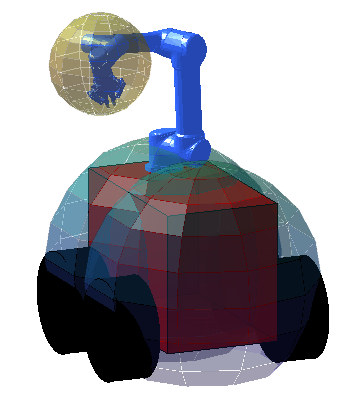
\includegraphics[scale=0.4]{IMMAGINI/spheres_3d.png}
	\caption{Spheres for self collision avoidance}
	\label{spheres_3d}	
	\end{figure}
	Formally the self collision avoidance constraint has been defined requiring that: 
	\begin{equation}
	\begin{split} 
		&\sqrt{({C_0}_x-{C_1}_x)^2+({C_0}_y-{C_1}_y)^2+({C_0}_z-{C_1}_z)^2} + r_1 +r_0 \geq 0 \\
		&\ \ \ \ \textnormal{and} \\
		&\sqrt{({C_0}_x-{C_2}_x)^2+({C_0}_y-{C_2}_y)^2+({C_0}_z-{C_2}_z)^2} + r_2 +r_0 \geq 0 \\
	\end{split}
	\label{spheres_const}
	\end{equation}
	where ${C_0}_{x,y,z},{C_1}_{x,y,z} \text{and }{C_2}_{x,y,z}$ are the coordinates of the centres of the end effector and base spheres, respectively, defined in the reference frame of the base and $r_1$ and $r_2$ are their radii. $r_0$ is the radius of the sphere encompassing the last joints of the arm and the EE, defined according to the physical dimensions as in \ref{spheres_3d} . This constraints definition introduces a nonlinear equation that has to be satiflied in the solution of the \ref{ourproblem_param}. \\

Summarizing, the presented constraints redefines the problem as:
\begin{equation} 
	\begin{split}
			& min_{p_k}\ J({x}_{k|0},p_k) = \sum_{i=1}^{N}\tilde{l}({x}_{k|i},p_k) \\
			\textnormal{s.t.}\qquad
			&\ \ \ \ x_{k|i+1}=\tilde{f}^+(x_{k|i},p_k,t_i) \\
			&\ \ \ \ {x}_{min}\ \leq\ x_{k|i}\ \leq\ {x}_{max}\  \forall\ i=1,\dots,\ N  \\
			&\ \ \ \ 0 \leq g^{sc}_{k|i}(x)\ \ \forall\ i=1,\dots,\ N \\
			&\ \ \ \ p_k\   \in \mathbb{P}\ \\
	\end{split}	
	\label{ourproblem_param_vinc}
\end{equation}
where $g^{sc}_{k|i}(x)$ is the function that defines the spheres constraints as in \ref{spheres_const}

